\section{Introduction}

Discrete diffusion models have become a powerful tool for molecular generation, such as for small molecules \citep{leeGenMolDrugDiscovery2025, schiffSimpleGuidanceMechanisms2025} and proteins \citep{wangDiffusionLanguageModels2024}, because they can model realistic chemical structures directly while producing diverse candidates.
In molecular design, however, unconditional generation is rarely useful. 
A pretrained generator $p_{\theta_0}$ encodes a broad molecular prior whose probability mass approximates the pretraining distribution, while a downstream design task defines a different target: sampling molecules achieving high rewards for a task-specific oracle $r(x)$. This oracle, which is typically costly to evaluate, might be a learned binding-affinity model \citep{jiangFlashAffinityBridgingAccuracySpeed}, a structure-prediction, a docking pipeline \citep{passaro2025boltz2}, or a wet-lab assay. Under a fixed evaluation budget, the typical goal of molecular optimization is to generate a molecule $x^*$ best-optimizing the given reward function:
\begin{equation}
    x^* \in \arg\max_{x \in \mathcal{X}} \; r(x) \label{eq:design_objective}
\end{equation}
where $\mathcal{X}$ denotes the valid chemical space under consideration.
% and generated samples $\mathcal{D_B} \coloneqq \{x_1, \ldots x_B\}$, the typical goal of molecular optimization is to maximize a utility $U(\mathcal{D}_B)$, defined over the set of evaluated molecules $\mathcal{D}_B$.  
% $$U(\mathcal{D}_B)=\max_{x\in\mathcal{D}_B} r(x)$$
% is the best molecule discovered; 
This formulation corresponds to top-$1$ discovery objective of the unknown reward function $r$, a problem also denoted by best-arm identification~\citep[e.g.,][]{lattimore2020bandit}. To tackle such generative optimization problems, the generator must be steered toward task-relevant regions of chemical space while preserving prior validity \citep{gutjahr2025constrained, HowArtificialIntelligence,  ueharaInferenceTimeAlignmentDiffusion2025}.
A powerful way to achieve this is via online model adaptation \citep{yangSteeringGenerativeModels2025, stoccoGuidingGenerativeModels2025, ueharaFeedbackEfficientOnline2024, rector-brooksSteeringMaskedDiscrete2024, suIterativeDistillationRewardGuided2025, ueharaRewardGuidedIterativeRefinement2025, yangSteeringGenerativeModels2025, stoccoGuidingGenerativeProtein2025, stoccoGuidingGenerativeModels2025, liCAGenMolConditionAwareDiffusion2026, olivecronaMolecularNovoDesign2017, blalockFunctionalAlignmentProtein2025}, as described next.



\textbf{Online Model Adaptation for Optimization:  Loop Structure.} 
\looseness -1 Given a pre-trained model, each round $t$ of online model adaptation alternates between two high-level steps (Fig.~\ref{fig:test_time_feedback}). A candidate pool $C_t$ of size $M$ is sampled from the current generator $p_{\theta_t}$, optionally with inference-time steering, and a batch $S_t$ of size $K$ is selected for oracle evaluation. The resulting pairs $(x,r(x))$ are appended to the evaluated set. Then the observed scores are converted into training rewards $\tilde{r}(x)$, optionally regularized, and used to update $p_{\theta_t}$ into $p_{\theta_{t+1}}$. Oracle feedback therefore has two roles: it determines the current discovery utility and, through model adaptation, changes which candidates the loop will propose in subsequent rounds.

% Crucially, while sampling molecules is generally cheap, oracle feedbacks are typically costly~\citep[][]{ueharaFeedbackEfficientOnline2024}.

% These evaluations can be expensive relative to sampling from the generator, so each oracle call must serve two roles: selecting useful candidate molecules now and providing feedback that can improve future generation.


%\textbf{A Tightly Coupled Design Problem.}
%\looseness -1 This setting yields a tightly coupled design problem. This includes how to select candidates for oracle evaluation, where strategies such as Thompson sampling can drive informative exploration~\citep[][]{ueharaFeedbackEfficientOnline2024, lattimore2020bandit}; and second, how to use oracle feedback to update the model, where reward shaping strategies such as top-$1$/$K$ objectives~\citep[e.g.,][]{santiFlowDensityControl, wang2026efficient} or model debiasing via negative score regularization~\citep[][]{de2025provable, santiFlowDensityControl, santiVerifierConstrainedFlowExpansion2026} can be employed. While these components have been studied separately, their interaction in online adaptation loops remains unclear. For instance, exploratory query selection may reduce the need for explicit debiasing, whereas aggressive top-$K$ shaping may make adaptation overly greedy. 

\textbf{A Tightly Coupled Design Problem.}
\looseness -1 The loop exposes tightly coupled choices that are often studied separately: which candidates receive oracle evaluations, how rewards are converted into model updates, and how the generator is pushed beyond biases in the pretrained prior. Previous works show that: Thompson sampling can improve oracle-call allocation through uncertainty-aware exploration~\citep[][]{ueharaFeedbackEfficientOnline2024, lattimore2020bandit}; top-$1$/$K$ or CVaR-style objectives can focus updates on the reward tail~\citep[e.g.,][]{santiFlowDensityControl, wang2026efficient}; and negative-score regularization can debias the generator away from over-occupied modes~\citep[][]{de2025provable, santiFlowDensityControl, santiVerifierConstrainedFlowExpansion2026}.
It is unclear whether these choices for acquisition, feedback reuse, reward shaping, and prior debiasing complement one another, become redundant, or interfere inside a full online adaptation loop.

To address this gap, we conduct an integrated study of representative design choices in online adaptation loops for discrete diffusion based molecule and protein optimization:

% This cost can be alleviated by learning a reward oracle surrogate, uncertainty estimates, or inference-time search to steer generation or prioritize candidates \needcite. In the second step, rewards can be reshaped to emphasize the upper tail, penalize invalid molecules, or encourage exploration beyond regions already favored by the current generator \needcite. The loop must also decide whether to train only on the latest batch or replay past evaluated molecules, how much fresh feedback to mix with retained high-reward samples, and how to prevent reward optimization from leaving the valid molecular manifold \needcite. Overall, a key question is what design choices to make to best allocate, reuse, and transform a limited stream of oracle feedback.

% We therefore perform an integrated study of online training loops for  molecular optimization using discrete diffusion. 

% Prior work has studied the main ingredients of this loop, including inference-time search with a fixed generator \citep{didi2026scaling, wangFineTuningDiscreteDiffusion2024, singhalGeneralFrameworkInferencetime2025, liDerivativeFreeGuidanceContinuous2024, nisonoffUnlockingGuidanceDiscrete2025, gruverProteinDesignGuided2023,  xiongProteinGuideOntheflyProperty2026, luProVADAGenerationSubcellular2025, ueharaRewardGuidedIterativeRefinement2025, liDynamicSearchInferenceTime2025, jianGeneralBindingAffinity2026, yangHitLeadDiscovery, tangPepTuneNovoGeneration2024, tangTR2D2TreeSearch2025, yangSteeringGenerativeModels2025}, online fine-tuning from scored samples \citep{rector-brooksSteeringMaskedDiscrete2024, suIterativeDistillationRewardGuided2025, ueharaRewardGuidedIterativeRefinement2025, yangSteeringGenerativeModels2025, stoccoGuidingGenerativeProtein2025, stoccoGuidingGenerativeModels2025, liCAGenMolConditionAwareDiffusion2026, olivecronaMolecularNovoDesign2017, blalockFunctionalAlignmentProtein2025}, and reward-guided diffusion objectives that turn oracle feedback into a training loss \citep{wangFineTuningDiscreteDiffusion2024, ueharaRewardGuidedIterativeRefinement2025, ueharaFeedbackEfficientOnline2024, santiFlowDensityControl, tangTR2D2TreeSearch2025, ueharaInferenceTimeAlignmentDiffusion2025}.  We ask how representative design choices around the objective interact: whether choices for acquisition, feedback reuse, reward shaping, prior debiasing, and validity control provide distinct value, reinforce one another, or become redundant once combined \needcite.


%Across $6$ small-molecule binding-affinity and $3$ protein fitness optimization tasks, our experimental results show that these mechanisms are complementary, particularly as high-reward solutions lie further outside the original generative distribution~\citep[][]{de2025provable, santiVerifierConstrainedFlowExpansion2026, jensen2025value}. In particular, debiasing via density entropy regularization  significantly improves exploration even when the acquisition function employed already accounts for reward-model uncertainty, showing that uncertainty in the reward model and bias in the generative prior are distinct bottlenecks. Similarly, reward shaping, replay, and validity control affect different parts of the training signal and failure profile rather than substituting for a stronger fine-tuning objective. 

\begin{figure}[t]
  \centering
    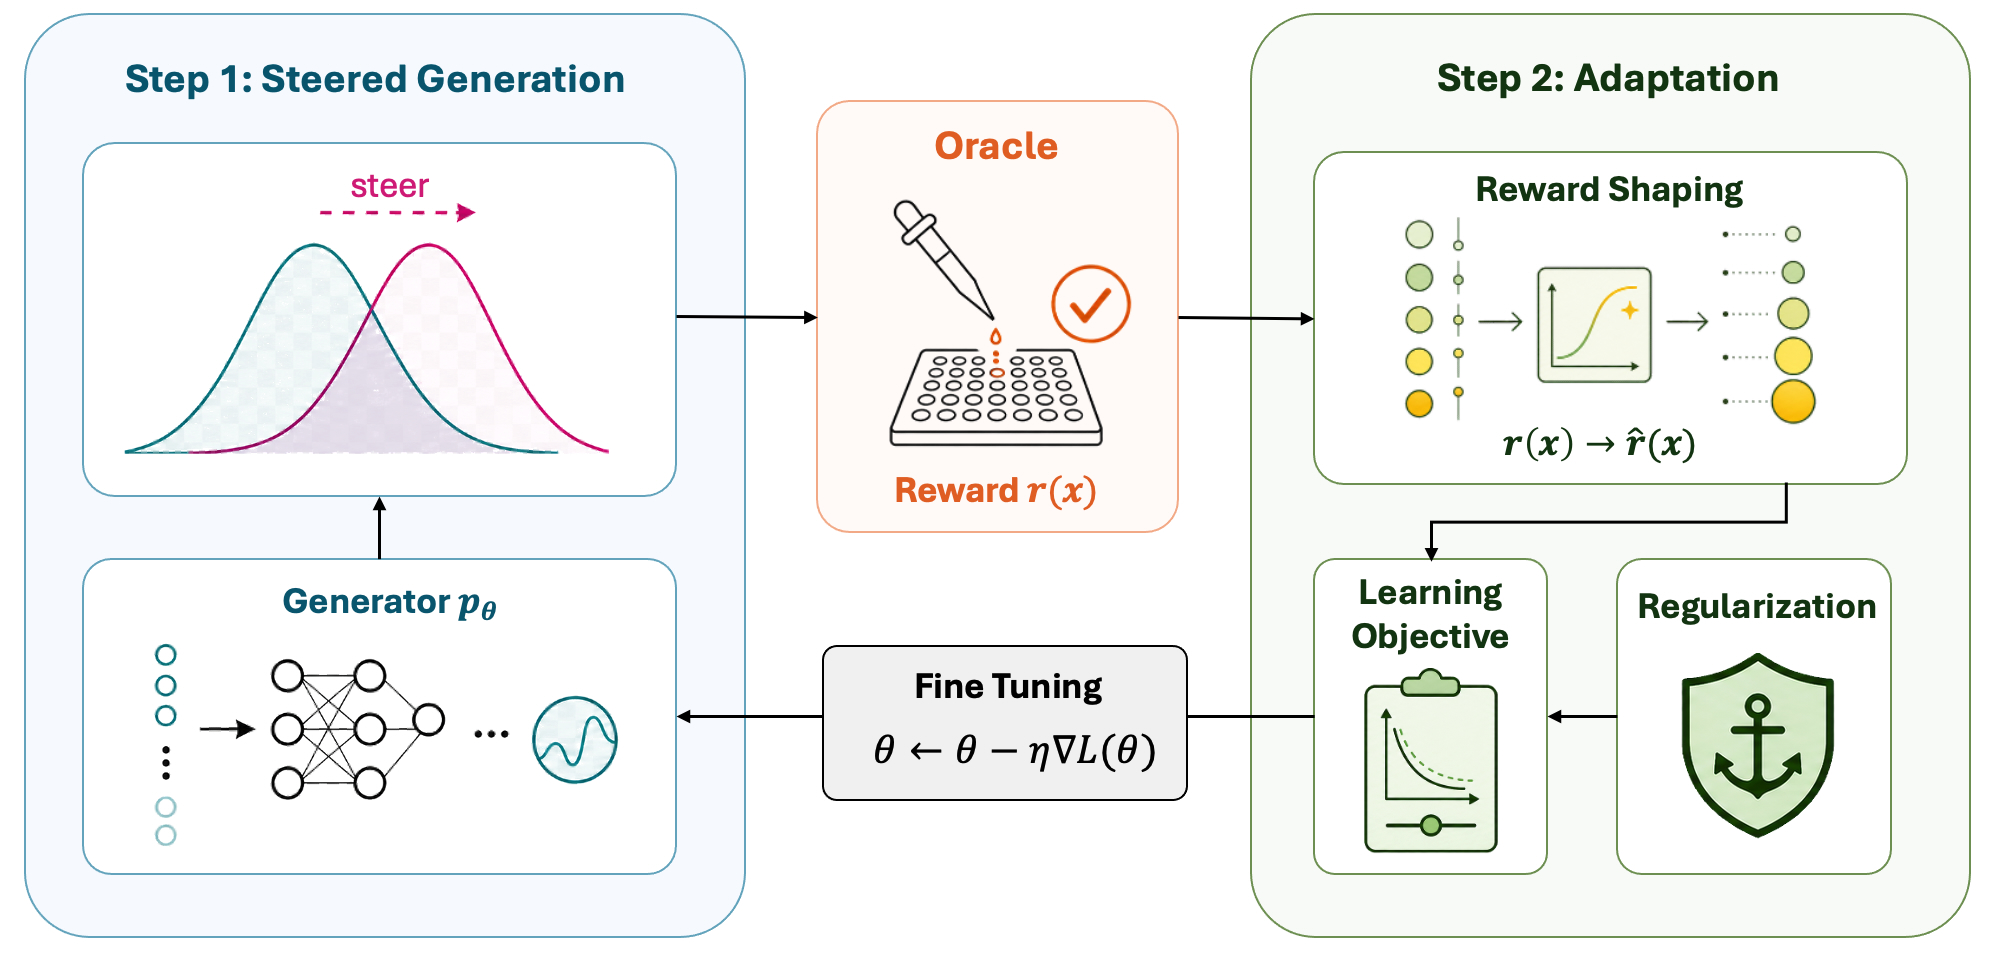
\includegraphics[width=\textwidth]{figures/overview.jpg}
    \vspace{-0.2in}
      \caption{\textbf{Online feedback loop for molecular optimization.}
Each round consists of two steps:
(1) the current generator $p_{\theta_t}$, updated using oracle feedback in Step~(2) of the previous round, generates candidates for the current round;
(2) the observed oracle rewards are converted into training signals to update the generator from $p_{\theta_t}$ to $p_{\theta_{t+1}}$.
The updated generator then returns to Step~(1), closing the online feedback loop.}
  \label{fig:test_time_feedback}
  \vspace{-0.1in}
\end{figure}


Our experiments on 9 tasks spanning small-molecule binding-affinity and protein-fitness optimization show that these mechanisms provide complementary benefits, especially when high-reward candidates have low likelihood under the pretrained generative prior. 
%In particular, density entropy regularization acts as model debiasing: it improves exploration even when acquisition already uses reward-model uncertainty, indicating that reward uncertainty and prior bias are distinct bottlenecks. Reward shaping, replay, and validity control likewise act on different parts of the loop: focusing updates on high-reward candidates, stabilizing learning over past feedback, and keeping exploration on the valid molecular manifold
On small molecules, acquisition, CVaR reward shaping, and Density Entropy Regularization provide the clearest complementary gains. On protein-fitness tasks, ablation effects are weaker, consistent with family-specific priors already covering high-fitness regions. Replay and validity control are primarily for keeping useful feedback across rounds and preventing exploratory updates from leaving the valid molecular manifold. 

\textbf{Overall, our contributions are: }
\begin{itemize}
    % \item We formulate test-time molecular optimization as an online feedback-allocation problem, where a fixed budget must be divided across candidate evaluation, reward modeling, replay, reward shaping, and generator updates.
    \item We provide a controlled empirical study of discrete-diffusion online adaptation for molecular optimization alongside offline fine-tuning and inference-time-search methods under fixed oracle and runtime budgets.

    \item We characterize the interactions among simple \emph{plug-in components} added to the online optimization loop through thorough ablations and mechanistic analysis: DER, CVaR, and Thompson Sampling exhibit compounding interactions while replay and validity control address distinct failure modes.

    \item We identify prior--reward mismatch as a useful diagnostic for when these mechanisms provide the most benefit. Under these observations, we assemble an online active fine-tuning recipe that substantially improves feedback efficiency over baselines.
    
    %We combine the best configurations of these components into a single online active fine-tuning recipe that outperforms all baselines at small-molecule and protein optimization under matched oracle-call budgets. We also elucidate that performance improvements are greater for molecular design solutions that lie further out of distribution from the original generative prior.
\end{itemize}